\chapter{Arrays of Arrays}

The last two chapters of this book will use 2D graphics to illustrate advanced object-oriented concepts.
If you haven't yet read Appendix~\ref{graphics}, please do so now to become familiar with the \java{Canvas}, \java{Color}, and \java{Graphics} classes from the \java{java.awt} package.
We will use these classes to make graphical programs.


\section{Conway's Game of Life}

A mathematician named John Conway invented the {\it Game of Life}, which he called a ``zero-player game'' because no players are needed to choose strategies or make decisions.
After you set up the initial conditions, you watch the game play itself.
That turns out to be more interesting than it sounds; you can read about it at \url{http://en.wikipedia.org/wiki/Conways_Game_of_Life}.

\begin{figure}[!ht]
\begin{center}
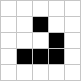
\includegraphics{figs/glider.png}
\caption{A ``Glider'' in the Game of Life.}
\label{fig:glider}
\end{center}
\end{figure}

The game consists of a two-dimensional grid of square cells.
Each cell is either ``alive'' or ``dead''; the color of the call indicates its status.
Figure~\ref{fig:glider} shows an example grid configuration.
The game proceeds in {\bf time steps}, during which every cell interacts with its {\bf neighbors} (adjacent cells).
At each step in time, the following rules are applied:

\begin{enumerate}
\item Any live cell with fewer than two live neighbors dies, as if by underpopulation.
\item Any live cell with more than three live neighbors dies, as if by overpopulation.
\item Any dead cell with exactly three live neighbors becomes a live cell, as if by reproduction.
\end{enumerate}

Notice some consequences of these rules.
If you start with a single live cell, it dies.
If all cells are dead, no cells come to life.
But if you have four cells in a square, they keep each other alive; that's a stable configuration.

Another stable configuration is shown in Figure~\ref{fig:blinker}.
Three horizontal cells become three vertical cells, which in the next time step become three horizontal cells, and the pattern continues forever.

\begin{figure}[!ht]
\begin{center}
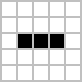
\includegraphics{figs/blinker-0.png}
\raisebox{38pt}{~$\longrightarrow$~}
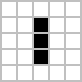
\includegraphics{figs/blinker-1.png}
\raisebox{38pt}{~$\longrightarrow$~}
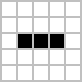
\includegraphics{figs/blinker-0.png}
\raisebox{38pt}{~$\longrightarrow$~ \ldots}
\caption{A ``Blinker'' in the Game of Life.}
\label{fig:blinker}
\end{center}
\end{figure}

Most simple starting configurations either die out quickly or reach a stable configuration.
But there are a few starting conditions that display remarkable complexity.
One of those is the R-pentomino: it starts with only five cells, runs for 1103 time steps, and ends in a stable configuration with 116 live cells (see
\url{http://www.conwaylife.com/wiki/R-pentomino}).

In the following sections, we will implement the Game of Life in Java.


\section{The Cell Class}

Using top-down design (see Section~\ref{shuffle}), it's pretty clear that we'll need at least three classes: one for the cells, one for the grid, and one for the game itself.
We'll begin by designing the class for cells.

When drawing a cell, we'll need to know its coordinates on the screen.
We could use a \java{Rectangle} object (see Section~\ref{sec:Rectangle}) to store the cell's coordinates.
However, given that each cell is a square, we can represent its location with only three integers: the \java{x} and \java{y} coordinates of the upper-left corner, and the \java{size} of the square (length of each side).
The cell will also need a \java{Color}.

Here is the beginning of the \java{Cell} class:

\begin{code}
public class Cell {
    private final int x;
    private final int y;
    private final int size;
    private Color color;
}
\end{code}

Notice that \java{x}, \java{y}, and \java{size} are constants.
Once the cell is created, we don't want it to move accidentally.
Its \java{color}, on the other hand, is not a constant and might change frequently.

The next step is to write a constructor.
It's good practice to design classes to be reusable, and there are other games that might need to make cells.
We'll make a constructor that takes \java{x}, \java{y}, and \java{size} as parameters.

\begin{code}
public Cell(int x, int y, int size) {
    this.x = x;
    this.y = y;
    this.size = size;
    this.color = Color.WHITE;
}
\end{code}

The following line uses the constructor to create a \java{Cell}.
Its upper-left corner is at (0, 0), and the cell is 10x10 pixels wide.

\begin{code}
Cell cell = new Cell(0, 0, 10);
\end{code}

To draw a cell, we will receive the graphics context as a parameter (similar to the \java{paint} method in Appendix~\ref{graphics}).
We then use \java{fillRect} to paint the cell itself and \java{drawRect} to paint a light gray border around it.

\begin{code}
public void draw(Graphics g) {
    g.setColor(this.color);
    g.fillRect(x + 1, y + 1, size - 1, size - 1);
    g.setColor(Color.LIGHT_GRAY);
    g.drawRect(x, y, size, size);
}
\end{code}

Finally, we will need methods for changing the cell's color.
We could just implement \java{getColor} and \java{setColor}.
But it will be more convenient if we design more specific methods.

For the Game of Life, the cells will either be dead (white) or alive (black).
To make the code more general, we will refer to these states as ``off'' and ``on''.
We will write boolean methods named \java{isOff} and \java{isOn} for getting the color, and void methods named \java{turnOff} and \java{turnOn} for setting the color.

%And to improve readability, we will define class constants for these colors.
%\begin{code}
%public static final Color OFF = Color.WHITE;
%public static final Color ON = Color.BLACK;
%
%public boolean isOff() {
%    return color == OFF;
%}
%public boolean isOn() {
%    return color == ON;
%}
%public void turnOff() {
%    color = OFF;
%}
%public void turnOn() {
%    color = ON;
%}
%\end{code}


\section{Two-Dimensional Arrays}

We can use an array to represent a grid of cells.
For example, we can represent a 5x5 grid with an array of 25 cells.
The following code is similar to how we created an array of cards in Section~\ref{cardarray}:

\begin{code}
Cell[] array = new Cell[25];
for (int r = 0; r < rows; r++) {
    int y = r * size;
    for (int c = 0; c < cols; c++) {
        int x = c * size;
        array[r * 5 + c] = new Cell(x, y, size);
    }
}
\end{code}

The loop variables \java{r} and \java{c} are the row and column indexes of each cell, and the variables \java{x} and \java{y} are the coordinates.
For example, if \java{size} is 10 pixels, then the cell at index (1, 2) would be at coordinates (10, 20) on the screen.

The expression \java{array[r * 5 + c]} calculates the index of the row and column in the array.
For example, the array index of the cell at (1, 2) would be 7.
Figure~\ref{fig:1D-array} illustrates how the rows are arranged.

\begin{figure}[!ht]
\begin{center}
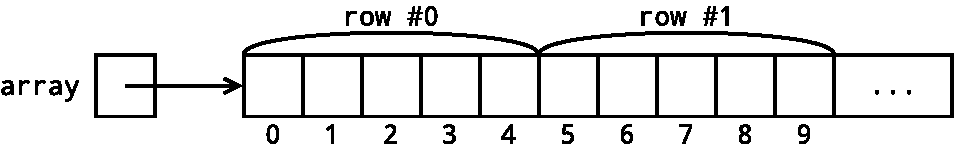
\includegraphics[width=366pt]{figs/1D-array.pdf}
\caption{Storing rows and columns with an array.}
\label{fig:1D-array}
\end{center}
\end{figure}

This way of represdenting two-dimensional data is know as {\bf row-major order}, because the elements are stored row by row.
A more natural way to represent {\bf multidimensional} data is to use multidimensional arrays, or arrays of arrays, as shown in Figure~\ref{fig:2D-array}.

\begin{figure}[!ht]
\begin{center}
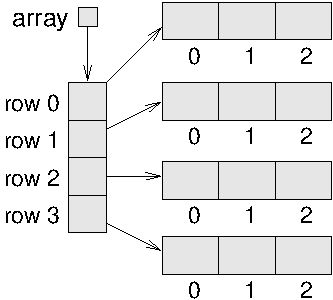
\includegraphics[width=265pt]{figs/2D-array.pdf}
\caption{Storing rows and columns with an array of arrays.}
\label{fig:2D-array}
\end{center}
\end{figure}

Using arrays of arrays makes it easier to refer to individual cells by row and column indexes.
We can rewrite the previous code by making two changes:

\begin{center}
\begin{tabular}{rl}
Replace: & \java{Cell[] array = new Cell[25];} \\[-1ex]
   With: & \java{Cell[][] array = new Cell[5][5];} \\[1ex]
Replace: & \java{array[r * 5 + c] = new Cell(x, y, SIZE);} \\[-1ex]
   With: & \java{array[r][c] = new Cell(x, y, SIZE);} \\
\end{tabular}
\end{center}

Notice that we no longer need to calculate the index \java{r * 5 + c}.
Instead, the expression \java{array[r]} gets the array at index \java{r}, after which \java{[c]} gets the cell at index \java{c}.


\section{The GridCanvas Class}

Now that we have a \java{Cell} class and a way of representing a two-dimensional array of cells, we can design a class to represent a grid of cells.
We will encapsulate the code from the previous section and generalize it to construct a grid of any size:

\begin{code}
public class GridCanvas extends Canvas {
    private Cell[][] array;

    public GridCanvas(int rows, int cols, int size) {
        array = new Cell[rows][cols];
        for (int r = 0; r < rows; r++) {
            int y = r * size;
            for (int c = 0; c < cols; c++) {
                int x = c * size;
                array[r][c] = new Cell(x, y, size);
            }
        }

        // set the canvas size
        setSize(cols * size, rows * size);
    }
}
\end{code}

\index{IS-A}
\index{HAS-A}

Using terminology from the previous chapter, \java{GridCanvas} ``is~a'' \java{Canvas} that ``has~a'' two-dimensional array of cells.
By extending the \java{Canvas} class from \java{java.awt}, we inherit methods for drawing cells on the screen.

In fact, that code is surprisingly straightforward.
To draw the grid, we simply draw each cell.
We use nested \java{for} loops to traverse the array of arrays:

\begin{code}
public void draw(Graphics g) {
    for (Cell[] row : array) {
        for (Cell cell : row) {
            cell.draw(g);
        }
    }
}
\end{code}

It's helpful to read the previous code in English: ``For each \java{row} in the grid \java{array}, and for each \java{cell} in the \java{row}, draw the \java{cell} in the graphics context.''
Each cell knows how to draw itself, because the coordinates are built-in.

The \java{Canvas} class provides two methods, \java{paint} and \java{update}, which are called to draw its contents.
These methods are intended to be overridden by the subclass to perform the actual painting and updating.
We will simply make them call the \java{draw} method, which paints or updates the entire Canvas.

%The default behavior of \java{paint} is simply to clear the \java{Canvas}; it's expected that a subclass will override this method.
%The default behavior of \java{update} is to clear the \java{Canvas} and then call \java{paint}.

\begin{code}
public void paint(Graphics g) {
    draw(g);
}
public void update(Graphics g) {
    draw(g);
}
\end{code}

In additional to \java{draw}, \java{paint}, and \java{update}, we will provide methods for working with the grid itself.
It will be useful to know how many rows and columns the grid has.
Fortunately this information is built into the array of arrays:

\begin{code}
public int numRows() {
    return array.length;
}
public int numCols() {
    return array[0].length;
}
\end{code}

Recall that \java{array} (the variable) is an array of rows.
So the number of rows is equal to the length of \java{array}.
Since the grid is rectangular, each row has the same number of columns.
So the number of columns is the length of \java{array[0]}, or any other row index for that matter.

Finally, we will write methods for working with individual cells.
The first method returns the \java{Cell} at (\java{r}, \java{c}), and the second method turns a \java{Cell} on.

\begin{code}
public Cell cellAt(int r, int c) {
    return array[r][c];
}
public void init(int r, int c) {
    array[r][c].turnOn();
}
\end{code}


\section{Starting the Game}

Now we can design a third class, named \java{Conway}, to implement the game itself.
\java{Conway} ``has~a'' \java{GridCanvas} that represents (and displays) the current state of the game.
The default constructor sets up an example board configuration.

\begin{code}
public class Conway {
    private GridCanvas grid;

    public Conway() {
        grid = new GridCanvas(5, 10, 20);
        grid.init(2, 1);
        grid.init(2, 2);
        grid.init(2, 3);
        grid.init(1, 7);
        grid.init(2, 7);
        grid.init(3, 7);
    }
}
\end{code}

This class will be the starting point of our application.
We will implement a \java{main} method to create a new window (\java{JFrame}), initialize the \java{grid}, and display it on the screen.
Doing so now will allow us to test \java{Cell} and \java{GridCanvas} before we implement the rest of the game.

\begin{code}
public static void main(String[] args) {
    String title = "Conway's Game of Life";
    Conway game = new Conway();
    JFrame frame = new JFrame(title);
    frame.setDefaultCloseOperation(JFrame.EXIT_ON_CLOSE);
    frame.setResizable(false);
    frame.add(game.grid);
    frame.pack();
    frame.setVisible(true);
}
\end{code}

Figure~\ref{fig:conway} shows the result of running the \java{main} method so far.
The \java{JFrame} has a title and is configured to exit the program when closed.
Resizing the window is disabled, and its only component is the game's \java{grid}.

\begin{figure}[!ht]
\begin{center}
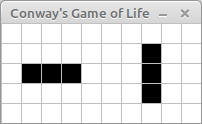
\includegraphics{figs/conway.png}
\caption{Screenshot of the initial Conway application.}
\label{fig:conway}
\end{center}
\end{figure}

At the end of \java{main}, we will add a \java{while} loop to simulate the time steps of the Game of Life.
During each time step, we will update the state of the \java{game} and repaint the \java{grid}.
This code is likely to execute very quickly, so we will use \java{Thread.sleep} to add a half-second delay (500 ms).

\begin{code}
while (true) {
    game.update();
    game.grid.repaint();
    
    Thread.sleep(500);  // compiler error
}
\end{code}

There's just one problem: compiling this code results in the error ``unreported exception InterruptedException''.
According to the documentation, \java{InterruptedException}


\section{Exception Handling}

Up to this point, the only exceptions we have seen are run-time errors like \java{ArrayIndexOutOfBoundsException} and \java{NullPointerException}.
When one of these exceptions occur, the program displays an message and terminates.

It's possible to ``catch'' these exceptions when they are ``thrown''.
In fact, some methods in the Java Library require you do handle exceptions that are likely to occur.
Such is the case with \java{Thread.sleep}; you may need to deal with sleep being interrupted.

To handle exceptions, you need to use \java{try} and \java{catch} blocks.
For example, we can try to sleep and do nothing if an \java{InterruptedException} occurs.

\begin{code}
try {
    Thread.sleep(500);
} catch (InterruptedException e) {
    // do nothing
}
\end{code}

Of course you can do something else when an exception is caught.
Or you can prompt the user to try again later.
In the case of our Game of Life program, it's not a big deal if the delay is slightly off.

There's a lot more to learn about exception handling that is beyond the scope of this book.
But you can read more about exceptions in the Java tutorials at \url{https://thinkjava.org/exceptions}.

Now that you know about \java{try} and \java{catch}, we can use them to implement a useful method in \java{GridCanvas}.
Part of the game's logic is to count the number of live neighbors.
Most cells have eight neighbors, as shown in Figure~\ref{fig:neighbors}.

\begin{figure}[!ht]
\begin{center}
\begin{tabular}{|p{1em}|p{1em}|p{1em}|p{1em}|p{1em}|}
\hline
  &   &   &   &   \\
\hline
  & 1 & 2 & 3 &   \\
\hline
  & 4 & * & 5 &   \\
\hline
  & 6 & 7 & 8 &   \\
\hline
  &   &   &   &   \\
\hline
\end{tabular}
\caption{Neighbors for a cell in the middle of the grid.}
\label{fig:neighbors}
\end{center}
\end{figure}

However, cells on the edges and in the corners have fewer neighbors.
If we try to count all eight possible neighbors, we'll go out of bounds.
(Normally in the Game of Life, we don't have this problem because the grid size is infinite.
But we thought that version might be a bit much for this chapter!)

We will write a helper method that tests whether a cell is alive.
If the \java{Cell} at (\java{r}, \java{c}) exists and is on, this method returns \java{1}.
Otherwise, it returns \java{0}.
The method can be used to count neighbors, regardless whether they exist.

\begin{code}
public int test(int r, int c) {
    try {
        if (array[r][c].isOn()) {
            return 1;
        }
    } catch (ArrayIndexOutOfBoundsException e) {
        // cell doesn't exist
    }
    return 0;
}
\end{code}

As before, this example does nothing when the exception is caught.
But doing so simplifies the code in the next section quite a bit.


\section{Finishing the Game}

The only remaining part to implement is the \java{update} method called by \java{main} in the \java{while} loop.
Each time step of the simulation consists of the following two actions (after getting the number of rows and columns):

\begin{code}
public void update() {
    int rows = grid.numRows();
    int cols = grid.numCols();

    // count neighbors before changing anything
    // update each cell based on neighbor counts
}
\end{code}

It's important to count {\em all} the neighbors first, before updating any cells, in order for the simulation to be correct.
We can define an array of arrays to store the neighbor counts:

\begin{code}
// count neighbors before changing anything
int[][] counts = new int[rows][cols];
for (int r = 0; r < rows; r++) {
    for (int c = 0; c < cols; c++) {
        counts[r][c] = countAlive(r, c);
    }
}
\end{code}

The \java{countAlive} method  invokes the \java{test} method we implemented in the previous section:

\begin{code}
private int countAlive(int r, int c) {
    int count = 0;
    count += grid.test(r - 1, c - 1);
    count += grid.test(r - 1, c);
    count += grid.test(r - 1, c + 1);
    count += grid.test(r, c - 1);
    count += grid.test(r, c + 1);
    count += grid.test(r + 1, c - 1);
    count += grid.test(r + 1, c);
    count += grid.test(r + 1, c + 1);
    return count;
}
\end{code}

If the \java{test} method didn't catch ``out of bounds'' exceptions, the \java{countAlive} method would have to ensure that \java{r} and \java{c} were in bounds.
Doing so would add many \java{if} statements to the code, making it more difficult to understand.

The second step of \java{update} is to change the state of each cell, based on its neighbor counts.
We simply traverse the rows and columns a second time:

\begin{code}
// update each cell based on neighbor counts
for (int r = 0; r < rows; r++) {
    for (int c = 0; c < cols; c++) {
        Cell cell = grid.cellAt(r, c);
        updateCell(cell, counts[r][c]);
    }
}
\end{code}

In contrast to the \java{draw} method of \java{GridCanvas}, which used enhanced \java{for} loops to traverse the array of arrays, this example uses standard \java{for} loops.
The difference here is that we need the indexes \java{r} and \java{c} to get the cell and its neighbor count.

Last but not least, the \java{updateCell} method implements the rules we defined at the beginning of the chapter:

\begin{code}
private static void updateCell(Cell cell, int count) {
    if (cell.isOn()) {
        if (count < 2 || count > 3) {
            cell.turnOff();
        }
    } else {
        if (count == 3) {
            cell.turnOn();
        }
    }
}
\end{code}

Notice that this method is \java{static}, because it does not depend on the \java{grid} attribute.
It is also \java{private}, because it is a helper method not intended to be invoked from outside the class.

If you put together and run the code from this chapter so far, you should see a simulation of two Blinkers.
More importantly, you will see a fairly complex example of object-oriented code that uses multidimensional arrays.


\section{Langton's Ant}

Now that we've finished the Game of Life, we can implement other zero-player games using \java{Cell} and \java{GridCanvas}.
One such game is {\it Langton's Ant}, which models an ``ant'' that walks around a grid of cells.
It displays surprisingly complex behavior based on two simple rules:

\begin{enumerate}
\item If the Ant is on a white cell, it turns to the right, makes the cell black, and moves forward.
\item If the Ant is on a black cell, it turns to the left, makes the cell white, and moves forward.
\end{enumerate}

Because the rules are simple, you might expect the ant to do something like make a square or repeat a simple pattern.
But starting on a grid with all white cells, the ant makes more than 10,000 steps in a seemingly random pattern before it settles into a repeating loop of 104 steps.
You can read more about it at \url{http://en.wikipedia.org/wiki/Langtons_ant}.

We begin by defining a \java{Langton} class that ``has~a'' grid and an ant.
The constructor takes the grid dimensions as parameters, which affect how long the simulation will run until the ant is out of bounds.

\begin{code}
public class Langton {
    private GridCanvas grid;
    private int xpos;
    private int ypos;
    private int head; // 0=North, 1=East, 2=South, 3=West

    public Langton(int rows, int cols) {
        grid = new GridCanvas(rows, cols, 10);
        xpos = rows / 2;
        ypos = cols / 2;
        head = 0;
    }
}
\end{code}

This class has essentially the same \java{main} method as \java{Conway}.
It sets up a \java{JFrame} and runs a simulation loop that calls \java{update}, \java{repaint}, and \java{sleep}.
However, we will only sleep for about 1~ms so that it runs a lot faster.

The \java{update} method is a lot simpler than before.
We first get the \java{Cell} at the ant's location, figure out which way to turn, and flip the cell's color.

\begin{code}
Cell cell = grid.cellAt(xpos, ypos);
if (cell.isOff()) {
    // at a white square; turn right and flip color
    head = (head + 1) % 4;
    cell.turnOn();
} else {
    // at a black square; turn left and flip color
    head = (head + 3) % 4;
    cell.turnOff();
}
\end{code}

Next, we move forward one square.
This is easily accomplished using chained \java{if} statements that determine which way the ant is facing.

\begin{code}
if (head == 0) {
    ypos -= 1;
} else if (head == 1) {
    xpos += 1;
} else if (head == 2) {
    ypos += 1;
} else {
    xpos -= 1;
}
\end{code}

If you run this code with a grid size of 61x61 or larger, you will see the ant eventually settle into a repeating pattern.


\section{Abstract Classes}

Looking back, the code for \java{Conway} and \java{Langton} are quite similar.
They each have a \java{GridCanvas}, an \java{update} method, and a \java{main} method.
Furthermore, the code for \java{main} is almost identical.

In the previous chapter, we learned how to eliminate two versions of the same code using inheritance.
We can apply a similar technique to \java{Conway} and \java{Langton}.
Doing so will make it easier to implement other zero-player games.

%Mathematically speaking, Conway's Game of Life and Langton's Ant are each a ``cellular automaton''.
%The word ``cellular'' means it has cells, and the word ``automaton'' means it runs itself.
%See \url{https://en.wikipedia.org/wiki/Cellular_automaton} for more discussion.

We will define a base class named \java{Automaton} to provide the code that \java{Conway} and \java{Langton} have in common.
Instead of \java{main}, it will have a \java{run} method that takes the window title and sleep delay as parameters.

\begin{code}
public class Automaton {
    private GridCanvas grid;

    public void update() {
    }

    public void run(String title, int delay) {
        // set up the window frame
        // main simulation loop
    }
}
\end{code}

There are a few problems with the current design:
\begin{enumerate}
\item The \java{grid} attribute is \java{private}, making it inaccessible in \java{Conway} and \java{Langton}.
We could add a \java{getGrid} method, but then other (unrelated) classes would have access to \java{grid}.
\item The \java{Automaton} class has no constructors, and even if it did, there would be no reason to create an instance of this class.
\item The \java{update} method does nothing, and in fact, it must be overridden for the \java{run} method to work correctly.
\end{enumerate}

Java provides language features to solve these problems:
\begin{enumerate}
\item We can make the \java{grid} attribute \java{protected}, which means it's accessible to subclasses but not other classes.
\item We can make the class \java{abstract}, which means it cannot be instantiated.
If you attempt to create an object for an abstract class, you will get a compiler error.
\item We can declare \java{update} as an \java{abstract} method, meaning that it must be overriden in subclasses.
If the subclass does not override an abstract method, you will get a compiler error.
\end{enumerate}

\begin{code}
public abstract class Automaton {
    protected GridCanvas grid;

    public abstract void update();

    public void run(String title, int rate) {
        // set up the window frame
        // main simulation loop
    }
}
\end{code}

Abstract classes are essentially incomplete (but useful) snippets of code that are intended to be reused in subclasses.
In the case of \java{Conway} and \java{Langton}, they make the code a lot cleaner.


\newpage
Table~\ref{tab:mainrun} summarizes major differences.

\begin{table}[!ht]
\begin{center}
\begin{tabular}{l|l}
\java{Conway.main}          & \java{Automaton.run} \\
\hline
\java{game.update();}       & \java{this.update();} \\
\java{game.grid.repaint();} & \java{grid.repaint();} \\
\end{tabular}
\caption{Comparison of \java{main} and \java{run} methods.}
\label{tab:mainrun}
\end{center}
\end{table}
